\documentclass[11pt]{beamer}

\usepackage[spanish]{babel}
\usepackage[utf8]{inputenc}


\usetheme{Copenhagen}
\setbeamercovered{transparent}


\title{Tres en raya con \textit{Raspberry Pi}}
\subtitle{Proyecto II}
\author{David Álvarez \and Guillermo Creus}
\institute[ETSEIB]{
  Escuela Técnica Superior de Ingeniería Industrial de Barcelona \\
  Universidad Politécnica de Cataluña
}
\date{\today}
\titlegraphic{
  
\includegraphics[height = 1.5cm]{Logo_ETSEIB.png}
  \hspace{1cm}
  
\includegraphics[height = 1.5cm]{Logo_UPC.png}
}



\begin{document}

\frame{\titlepage}

\begin{frame}{Índice}
  \begin{columns}
    \column{.5\textwidth}
    \tableofcontents
    \column{.45\textwidth}
    \begin{figure}[h]
      \centering
      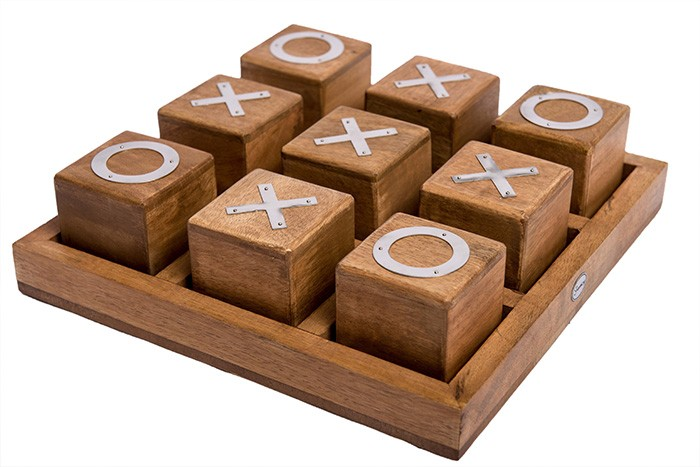
\includegraphics[width = \textwidth]{tic-tac-toe.jpg}
      \caption{Tres en raya.}
      \label{fig:tic-tac-toe}
    \end{figure}
  \end{columns}
\end{frame}


\section{Introducción}

\subsection{Idea inicial}
\begin{frame}{Idea inicial}
  \begin{columns}
    \column{.50\textwidth}
    \begin{itemize}
    \item Brazo robótico
    \item 3 en raya
    \end{itemize}
    \column{.50\textwidth}
    \begin{figure}[h]
      \centering
      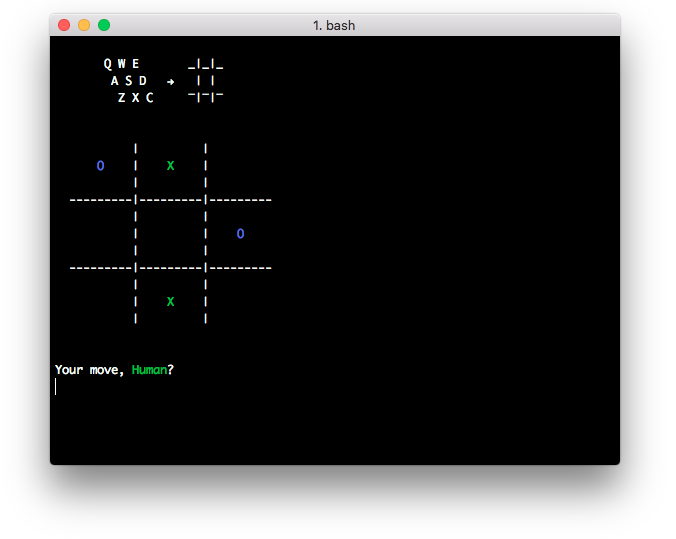
\includegraphics[width=\textwidth]{terminal.png}
      \caption{Interfaz Brazo robótico - Ordenador}
      \label{fig:terminal}
    \end{figure}
  \end{columns}
\end{frame}


\section{El proyecto}

\subsection{Etapas}
\begin{frame}{Estructura del proyecto}
  \begin{block}{Programación}
    \begin{itemize}
    \item Programa capaz de realizar movimientos tras la inserción de una jugada
    \item Conexión Ordenador, Raspberry y brazo robótico
    \end{itemize}
  \end{block}

  \begin{alertblock}{Mecánica}
    \begin{itemize}
    \item Control movimiento del brazo
    \item Accionamiento pinza
    \end{itemize}
  \end{alertblock}
\end{frame}

\begin{frame}{Futuro}
  \begin{itemize}
  \item Detección del movimiento de las piezas usando una cámara.
  \item ¿Otros juegos...?
  \end{itemize}
  \vspace{.5cm}
  \begin{figure}[h!]
    \centering
    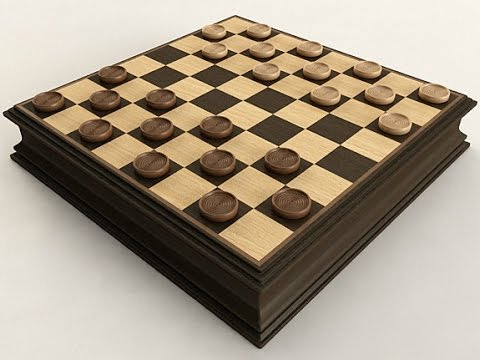
\includegraphics[height = 3cm]{damas.jpg}
    \hspace{1cm}
    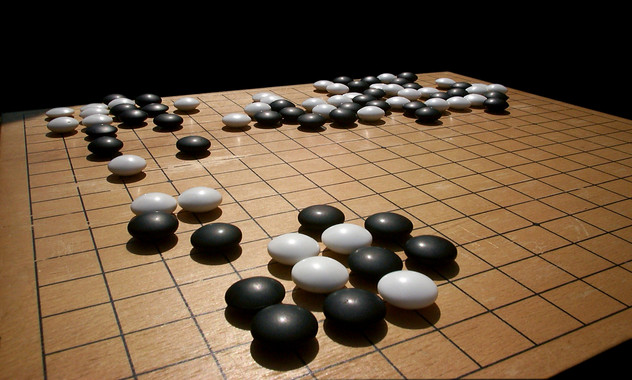
\includegraphics[height = 3cm]{go.jpg}
    \caption{Otros posibles juegos.}
  \end{figure}
\end{frame}

\begin{frame}
    \begin{center}
        Gracias por la atención.
    \end{center}
\end{frame}

\end{document}
